% Chapter 1

\chapter{Egocentric Vision and Wearable devices: an overview}

\lhead{Chapter 1. \emph{Wearable devices and new human-machine interfaces}} % This is for the header on each page - perhaps a shortened title

%----------------------------------------------------------------------------------------

\section{Introduction}

Portable head-mounted cameras, able to record dynamic high quality first-person videos, have become a common
item among sportsmen over the last five years. These devices represent the first commercial attempts to record
experiences from a first-person perspective. This technological trend is a follow-up of the academic results
obtained in the late 1990s, combined with the growing interest of the people to record their daily activities.
As a recent survey on first person vision \cite{surveyfpv} recalls, the idea of recording and analyzing videos from first person perspective is not new. To mention some examples:
In 1998 Mann proposed the WearCam \cite{mann1998wearcam}. Later in 2000, Mayol \etal proposed a necklace device \cite{mayol2002wearable} , and in 2005 Mayol et al. developed an active shoulder mounted camera \cite{mayol2005applying}. In 2006, the Microsoft Research Center started to use the SenseCam for research purposes \cite{hodges2006sensecam}, while Pentland \etal \cite{blum2006insense} developed a wearable data collector system (InSense). Finally, it is important to
highlight the work of Mann, who, since 1978, has been working on his own family of devices. 

Up to date, no consensus has yet been reached in the literature with respect to naming this video perspective.
\textit{First Person Vision} (FPV) is probabily the most commonly used term, but also \textit{Egocentric Vision}
has also recently grown in popularity, and will be used in the rest of this thesis.  In the awakening of this technological trend, Google announced the Project Glass in 2012. The company started publishing short previews on the Internet demonstrating
the Glasses FPV recording capabilities. This was coupled by the ability of the device to show relevant information to the user through the head-up display. The main idea of the Project Glass is to use a wearable computer to reduce the time between intention and
action. In this thesis, we try to move a step forward, and realize a wearable vision device with better computing capacities and thus able to execute complex computer vision algorithms.

\section{On the positioning of the camera}
The ego-centric approach consists in equipping the users with wearable sensors that observe their activities: these devices see what the user sees and look where the user is looking. One of the first questions to solve, of course, is where to put the camera. Positioning an optical device on the human body is quite a problematic task, as occlusion, motion, social issues as well as criteria related to the purpose of the device must be taken into account. Following the work of Mayol \etal \cite{mayol2001positioning}, in this section we give a detailed overview on the best places where to put a wearable camera.

Cameras used for wearable applications fall into two categories for this discussion; static narrow-view devices and omnidirectional devices. Omnidirectional devices include catadioptric, fish-eye and active systems where either the entire field-of-viewis imaged at low resolution, or in the active case the high-resolution narrow-view sensor moved to any orientation. Narrow-view static cameras can only ever see a small part of the user or their environment, and placement is therefore entirely driven by the task. For wide-angle or omnidirectional sensors placement is less constrained and a range of positions are possible. 

A variety of solutions appear in the literature. In \cite{starner1998real, schiele1999attentional}, hat-mounted cameras have been used to look down at the user’s hands and reaching space, whereas in \cite{kohtake1999infostick} cameras are strapped to the wearer’s hands themselves. In \cite{aoki1999realtime}, a hat-mounted camera looks forward, an orientation also used when the camera is attached to a head mounted display \cite{mann1998wearcam}. In contrast, \cite{starner2000gesture} uses a camera worn on the chest, in \cite{rungsarityotin2000finding} an omnidirectional camera is used above the head, and a wide-angle lens camera mounted at the back in \cite{clarkson1999unsupervised}.

Mayol \etal \cite{mayol2001positioning} identify three frames of reference for measurements that a wearable sensor makes: 
\begin{enumerate}
\item relative to the user body (e.g. sensing the manipulative space in front of the user’s chest)
\item relative to the static world (e.g. sensing the ceiling/floor texture to infer user’s location)
\item relative to an independent object (e.g. tracking an interesting object)
\end{enumerate}
This task-oriented classification can help us to understand the criteria that should be considered. For working in the user frame alone all that is required is a stable view of the chosen area — often the handling space, and absolute field-of-view may be less important. For sensing the outside environment user occlusion is problematic and absolute field-of-view is more important. Both occlusion and
user motion are problems when fixating resolution or processing on a particular part of the environment or independently moving object.

To simulate and compare positions for optical devices around a human body, we must first simulate the human form: \cite{mayol2001positioning} use a female example from the Human Animation Working Group\footnote{\url{http://www.h-anim.org}}, consisting of about 1000 markers (points) and 1800 polygons arranged into 16 body-segments which can be independently rotated to simulate any natural pose. They have created a software\footnote{freely available at \url{http://www.robots.ox.ac.uk/~wmayol/3D/nancy_matlab.html}} to allow the simulated optical device to be positioned arbitrarily in space around the body, or for faster automatic tests placed a distance above any of the humanoid’s polygons. The utility of such a model is that the variables of position and distance above the body-surface can be varied automatically, allowing tests for a range of device heights over the whole body (which would be tedious at best on a real person).

Determination of occlusion in any direction can be made by emitting a ray from the chosen device centre and checking for intersection with any of the component polygons. Only polygons facing the camera need be considered, and refinements to further reduce the number of tests are widely reported in the ray-tracing literature. For visualization it is also useful to consider emitting rays from the device centre as equivalent to a central projection onto a unit sphere. This yields representations such as Figure \ref{fig:Positioning1}, where
the head is clearly visible to the right with the shoulder below it. The proportion of the sphere surface not occluded gives the absolute field-of-view.

\begin{figure}[htbp]
	\centering
		\includegraphics[page=3]{Figures/mayol_etal_ouel224101_cropped.pdf}
	\caption{Left: The device is positioned above the centroid of the polygon, a short distance (37.5mm) along the surface normal. Right: The view from such a camera shows the head and shoulder clearly, but the rest of the body is obscured.}
	\label{fig:Positioning1}
\end{figure}

In terms of absolute field of view, the head, the position of choice for many researchers (and nature), is favourable, as are the
shoulders. This comes as no surprise: however it is important to note which alternative placements are favorable if these locations can not be used (e.g. for social reasons). A further consideration is that raising the sensor away from the body might reduce the occlusion. Figure \ref{fig:Position2} shows the amount of occluision in some of the favoured positions and varies the sensor height from resting on the surface (height=0mm) to far above (height=150mm). At all of the chosen positions the occlusion reduces as the height is increased, but the most significant gains are made for the head-mounted positions and shoulder area. Whichever position is chosen, the field of view is always significantly improved if the sensor can be raised a few centimeters from the surface. However, increases beyond 50mm make no significant improvement in the field of view for this model.

\begin{figure}[htbp]
	\centering
		\includegraphics[page=4]{Figures/mayol_etal_ouel224101_cropped.pdf}
	\caption{The proportion of the view obscured against the distance from the body.}
	\label{fig:Position2}
\end{figure}

The amount of usermotion must also be taken into account. The type of motion that may be encountered can vary enormously and
may be task dependent. With an articulated model it is possible to analyze any motion for which the joint angle evolutions over time are known. In figure \ref{fig:Position3}, we show the amount of motion . The arms and legs suffer the highest
motions, with most of the torso and head relatively still.

\begin{figure}[htbp]
	\centering
		\includegraphics[page=8,width=0.4\linewidth]{Figures/mayol_etal_ouel224101_cropped.pdf}
	\caption{Amount of motion: arms and legs suffer the most severe motions during walking.}
	\label{fig:Position3}
\end{figure}

Now, having considered and evaluated occlusion, motion, and distance, it is clear that the best places to put a wearable camera, with respect to these parameters, are head and shoulders. Of course, an head mounted camera will suffer a bigger motion, but can reveal attentional cues, and it is thus the best choice for action and activity recognition. Shoulder mounted cameras, on the other hand, are less invasive, and are still a good choice for social interaction analysis and human-machine interfaces. In this thesis we will explore both options.

\section{Wearable devices}
The term \textit{wearable device} refers to electronic technologies or computer that are incorporated into items of clothing and accesories which can be worn on the body. In our case, we are mainly interested in developing wearable \textit{vision} devices, i.e. wearable devices capable to see and process video data. In this section, we will provide a brief description for some of these devices and our experience in using a few of them.

\subsection{Go-Pro}
GoPro offers a series of small and high-quality cameras. These cameras can be mounted on various
body parts or objects such as a helmet, chest and snow board which makes them very flexible. The
GoPro Hero 1 has a fish-eye lens with a 110 view angle. The view angle has increased to 170 in
the more recent Hero 2 and 3 cameras. The quality of the video is in HD, with minimal motion
blur and other artifacts. The quality of the video is much better outdoors, and the video sometimes
becomes very dark indoors. The main advantage of the GoPro camera is its wide field of view
and its high quality video. On the other hand, its disadvantage is its bulkiness, and the fact that
other individuals in the scene become very aware of it. The battery lasts for about 2 hours during
continuous video capture. The data is recorded on a SD card. A 16GB SD card suffices for storing
2 hours of HD video. The price of GoPro is around 200\$.

\subsection{Tobii Eye-Tracking Glasses}
Tobii offers various kinds of eye-tracking products. Most of their devices are static and monitorbased.
However, they have a few mobile eye-tracking systems as well. The system consists of an
outward looking camera that captures the scene in front of the user, and an inward looking infrared
camera that tracks the subject’s right eye. The glasses connect to a pocket size recording device.
Before or after data collection, the system needs to be calibrated in order to correctly estimate the
gaze point. Calibration is very intensive and becomes very hard for some subjects. The resolution
of the video is $640\times480$ and the frame rate is 30 fps. The video quality is low and there exist severe
motion blur and interlacing effects. On the plus size, the gaze tracking is accurate in comparison
to the wearable gaze-tracking devices of other companies. The view field of the camera is around
$600\times400$. The price of Tobii eye-tracking glasses is around 30,000\$.

\subsection{SMI Eye-Tracking Glasses}
SMI produced a device similar to Tobii’s eye-tracking glasses in January 2012. They have tried to fix some of the issues that exist in the Tobii’s system. In particular, their system is easier to calibrate, records a video in HD, and the glasses are more tolerable on the face. The SMI system has two eye-tracking infrared cameras looking at both eyes which results in an easier calibration in comparison to Tobii’s system. An issue that exists in the SMI glasses is that the video is blurred and dark on the frame boundaries. The price
of SMI eye-tracking glasses is around 24,000\$.

\subsection{Pivothead Glasses}
Pivothead has introduced a relatively cheap pair of glasses that have an outward looking camera
that captures the scene in front of the user. Obviously this is a cheaper system in comparison to
SMI and Tobii because it doesn’t track the eyes. The video quality is HD and it can capture for an
hour. The only issue with the pivothead glasses is that the camera’s field of view is very narrow,
even narrower than that of SMI and Tobii systems. The price of Pivothead glasses is around 300\$.
They also provide a 100\$ device which can transmit video to a laptop in realtime.

\subsection{Google Glass}
Google Glass is about to become available for public use. The system records a 720p video and
takes 5-megapixel images. It can connect to the internet and any bluetooth-capable phone. In
addition, Glass has a heads up display (HUD) creating an illusion equivalent to viewing a 25-inch
high definition screen from eight feet away. It has 16 GB of RAM, 12 GB of which are usable for
apps. Furthermore, it has a microphone, similar to all of the previously mentioned wearable devices.

\subsection{Panasonic HX-A10}
\label{panasonic}
The Panasonic HX-A10, rather than relying on mounts and accessories, is equipped with an ''earhoo'' feature and a remote processing unit, which allows users to attach the camera to their head right out of the box, and no helmet is required. The device itself records at $1920\times1080$ video at 60 fps, $1280\times 720$ at 120 fps, and $640\times360$ at 240 fps for slow shots. It has Wi-Fi and can setup a live stream; and battery life for over two hours of filming on a single charge.

The actual lens (F2.5 bright lens, 1/4.1-inch BSI Sensor) part sports a two-foot cable and only weighs in at 4 ounces. It also communicates with a smartphone or tablet while watching in live view. We used the Panasonic HX-A10 to record two datasets, the Interactive Museum dataset and the Maramotti dataset, taken into the Maramotti Collection (Figure \ref{fig:Panasonic}). The lens helps to capture a wide field of view, which is necessary for observing first-person’s hands during daily activities. The fish-eye distortion, however, creates some challenges for using the data.


\begin{figure}[htbp]
	\centering
		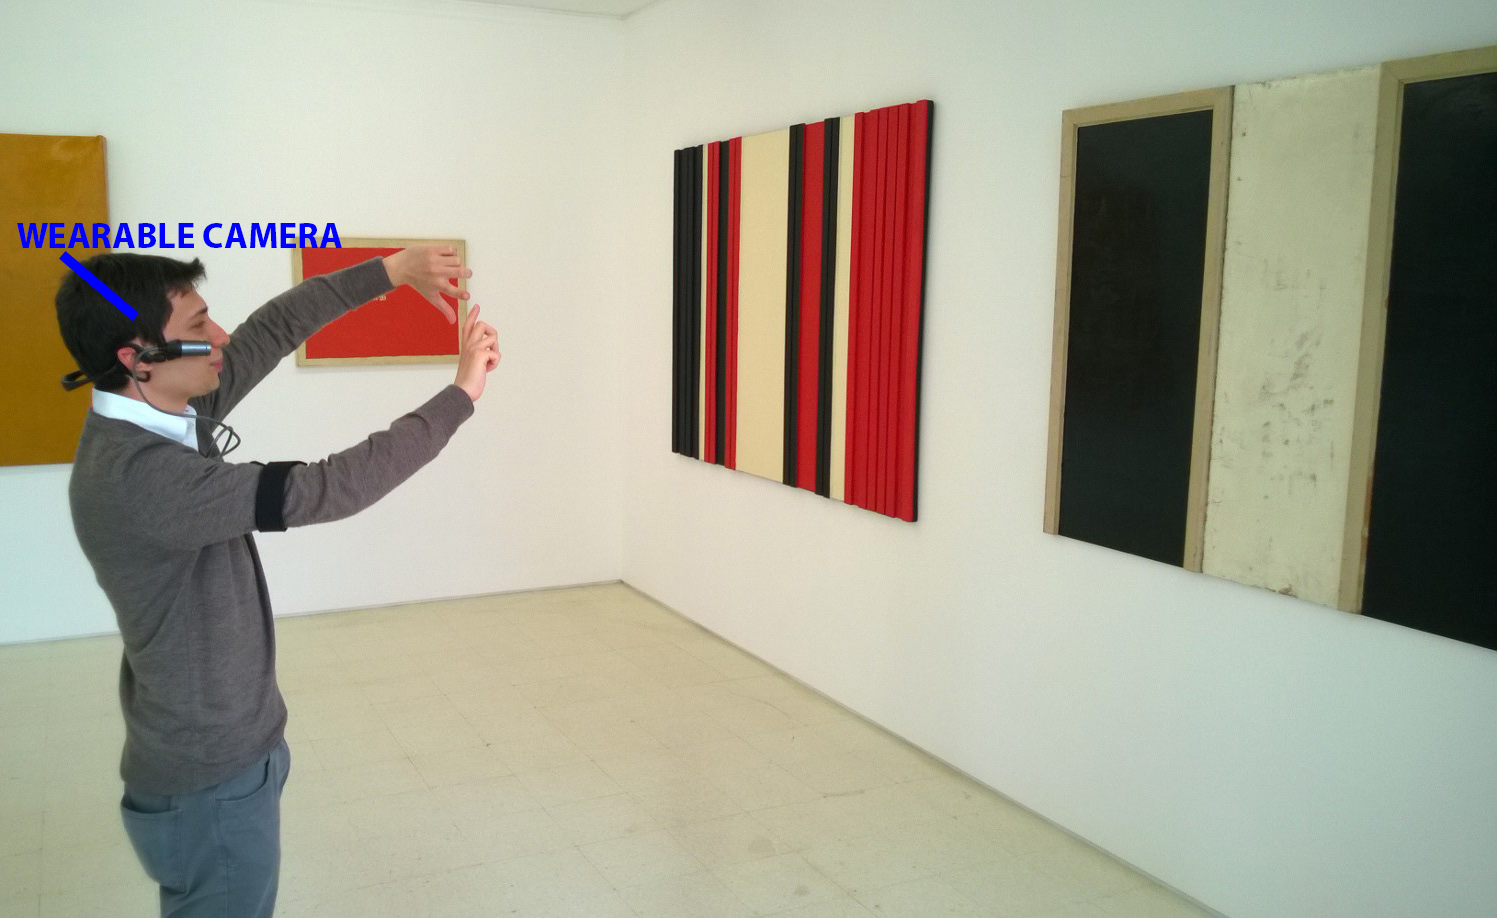
\includegraphics[width=0.4\linewidth]{Figures/lore_maramotti.jpg}
	\caption{We used Panasonic HX-A10 for collecting the Interactive Museum dataset and the Maramotti dataset.}
	\label{fig:Panasonic}
\end{figure}

\subsection{Genius WideCam F100}
The Genius WideCam F100\footnote{\url{http://www.geniusnet.com/Genius/wSite/ct?xItem=53214&ctNode=161}} is a wide angle HD camera that we used in some of our tests, and is the camera mounted on our wearable vision device. It can record 1080p frames at up to 30 fps and features ultra wide angle lens (up to 120 degrees) and built-in microphones (see figure \ref{fig:wide-camera}).

\begin{figure*}[tb]
\centering
\subfigure[]{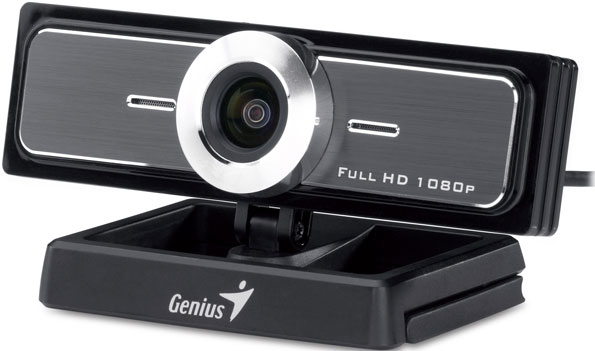
\includegraphics[height=100px]{./Figures/WideCam_F100_Angle.jpg}}
\subfigure[]{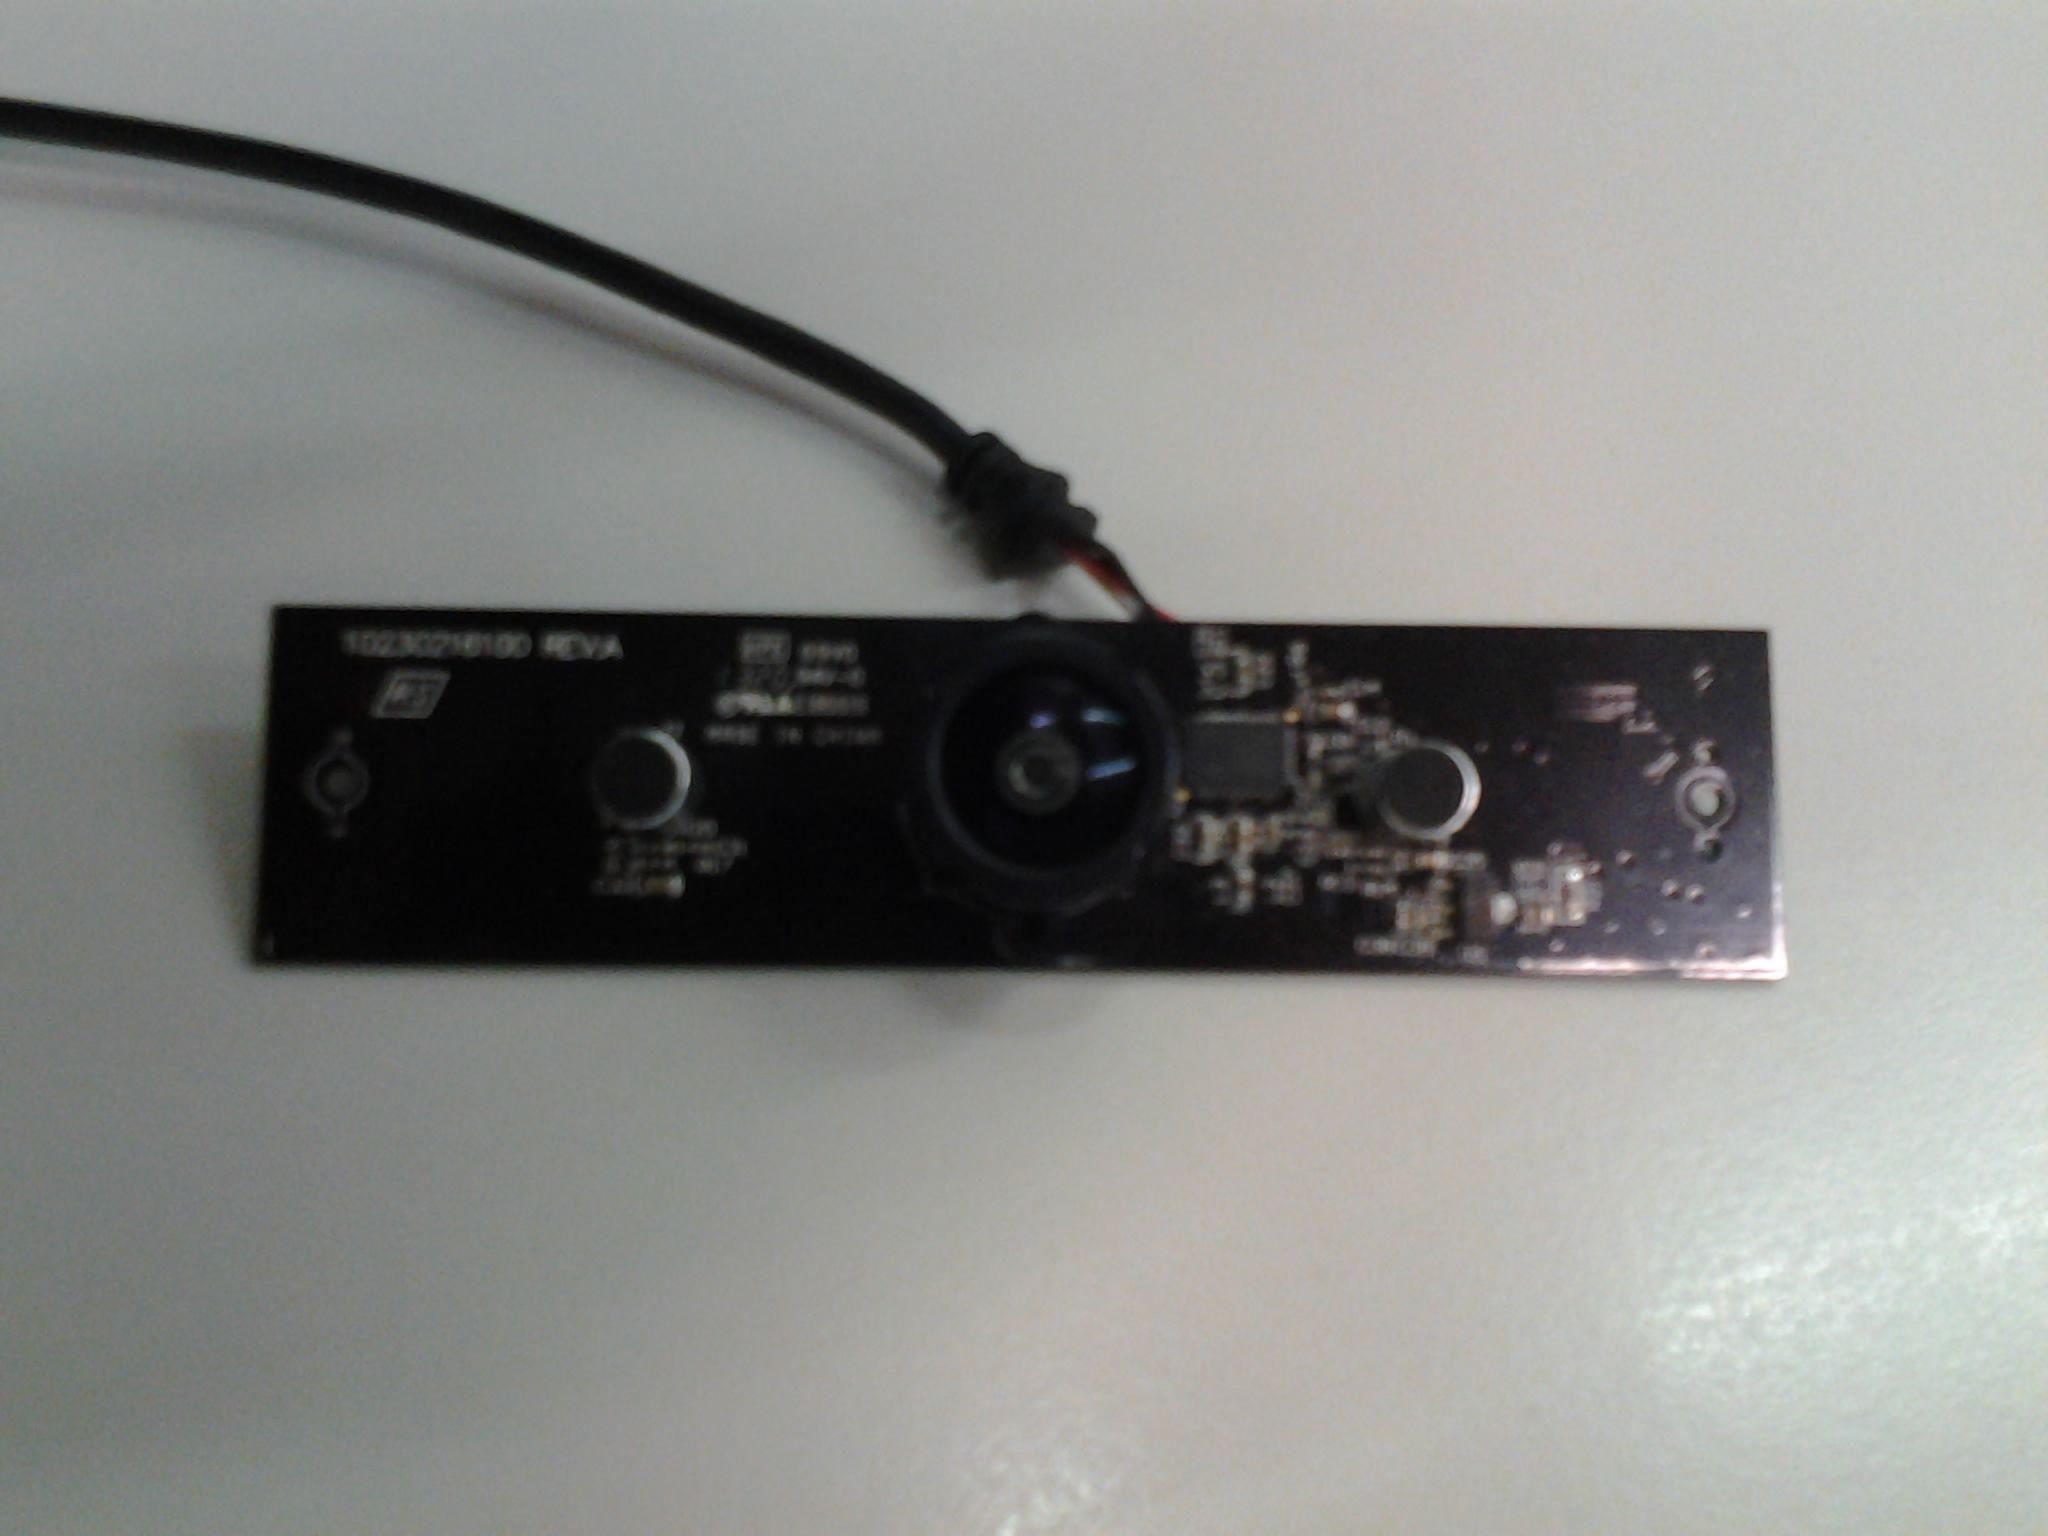
\includegraphics[height=100px]{./Figures/wide_camera.jpg}}
\caption{Genius WideCam F100.}
\label{fig:wide-camera}
\end{figure*}

\subsection{The Odroid-XU board}
\label{odroid-intro}
The wearable ego-vision devices we have built embe a glass-mounted camera and an Odroid-XU developer board, serving as video-processing and network communication unit.
There are several benefits in using such a portable device: the commercial availability and low costs for prototypes evaluation, the computational power and energy efficiency of the Big-Little architecture. Furthermore it has the possibility  of peripheral addition to extend connections and input devices. 

\begin{figure}[t!]
\centering
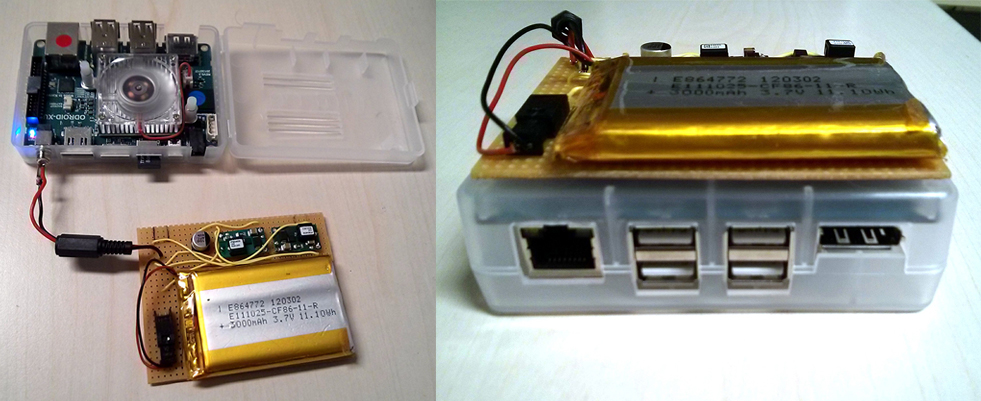
\includegraphics[width=0.6\linewidth]{Figures/board.jpg}
\caption{The Odroid-XU board with battery pack.}
\label{board}
\end{figure}

Hardkernel have made a name for themselves within the open-source community by delivering high performance development boards at affordable prices. The Odroid-XU platform boasts an Exynos 5 Octa processor – the same SoC found inside the Samsung Galaxy S4, which includes a PowerVR SGX544MP3 GPU clocked at around 600 MHz (see figure \ref{odroid-xu}).

The key features and specifications of the ODROID-XU development board include:
\begin{itemize}
\item big.LITTLE processing based on the Cortex™-A15 and Cortex™-A7 quad core CPUs
\item PowerVR SGX544MP3 GPU (OpenGL ES 2.0, OpenGL ES 1.1, OpenCL 1.1 EP, Renderscript/Filterscript)
\item 2Gbyte LPDDR3 PoP (1600Mbps/pin, 2 x 32bit Bus)
\item USB 3.0 Host x 1, OTG x 1, USB 2.0 Host x 4
\item HDMI 1.4a output Type-D connector (Micro-HDMI)
\item eMMC 4.5 Flash Storage
\item Micro-SD socket
\item MIPI DSI for LCD display output
\item On-board Audio Codec
\item Fast 10/100 Ethernet LAN
\item WiFi
\item 5V/4A power supply
\end{itemize}

Big.LITTLE is a heterogeneous computing architecture developed by ARM that couples slower, low-power processor cores with more powerful and power-hungry ones. The intention being to create a multi-core processor that can adjust better to dynamic computing needs and use less power than clock scaling alone. In this case we have the Cortex-A7 coupled with the Cortex-A15, which have been designed to be architecturally compatible.

In the Samsung Exynos 5 there is only one way for the different processor cores to be arranged in a big.LITTLE design: the \textit{clustered model} approach. With this approach the operating system scheduler can only see one of the two processor clusters, when the load on one cluster hits a certain point, the system transitions to the other cluster. All relevant data is passed through the common L2 cache, the first core cluster is powered off and the other one is activated. A Cache Coherent Interconnect (CCI) is used.


%----------------------------------------------------------------------------------------
\section{Previous work in Egocentric Vision}
We now discuss the relationship between this work with other areas of related work. Egocentric vision is an emerging area in computer vision. Every year around ten papers addressing this topic appear in top vision conferences (CVPR, ICCV and ECCV). It is possible to categorize these papers into roughly three main groups:
\begin{itemize}
\item Recognition of Activities
\item Gaze in Egocentric Vision
\item Day-long Video Summarization
\end{itemize}

In this chapter, we describe the related work to each of these topics.



%----------------------------------------------------------------------------------------
\section{About this thesis: gestures}
As we said before, the main aim of this thesis, from the hardware point of view, is to develop a wearable vision device capable of executing intensive computer vision algorithms. From the software point of view, we would like to build a new human-computer interface based on gestures: for example gestures are used to control a wearable vision device that lets the user interact with artworks (Figure \ref{fig:interaction}).

\begin{figure*}[tb]
\centering
\subfigure[]{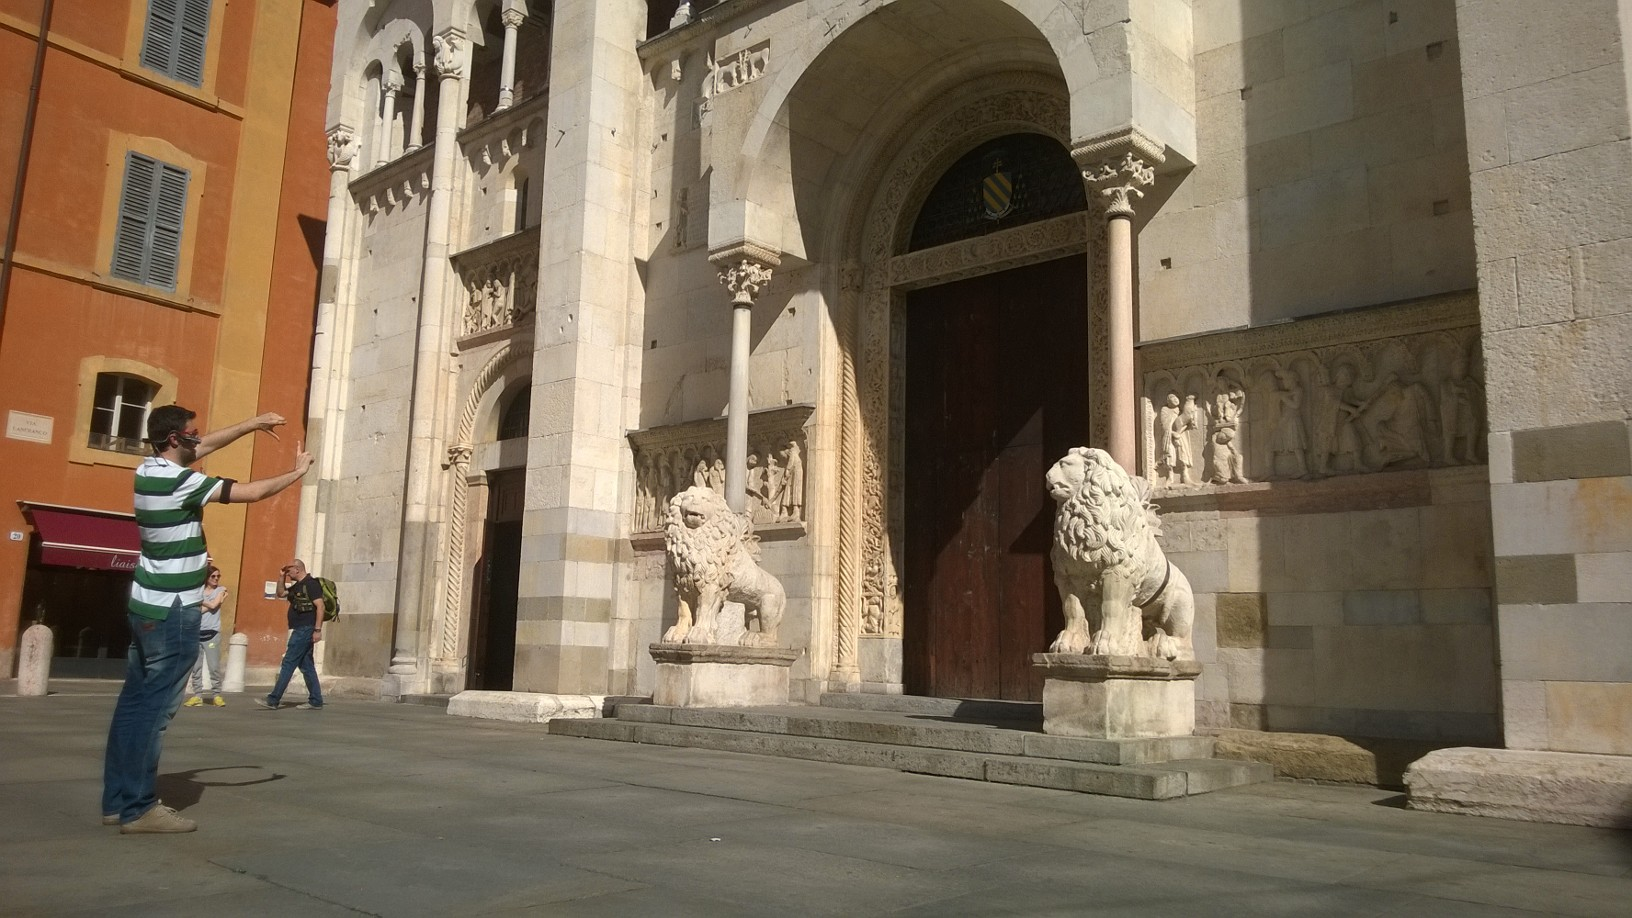
\includegraphics[height=100px]{./Figures/egovision_duomo_modena.jpg}}
\subfigure[]{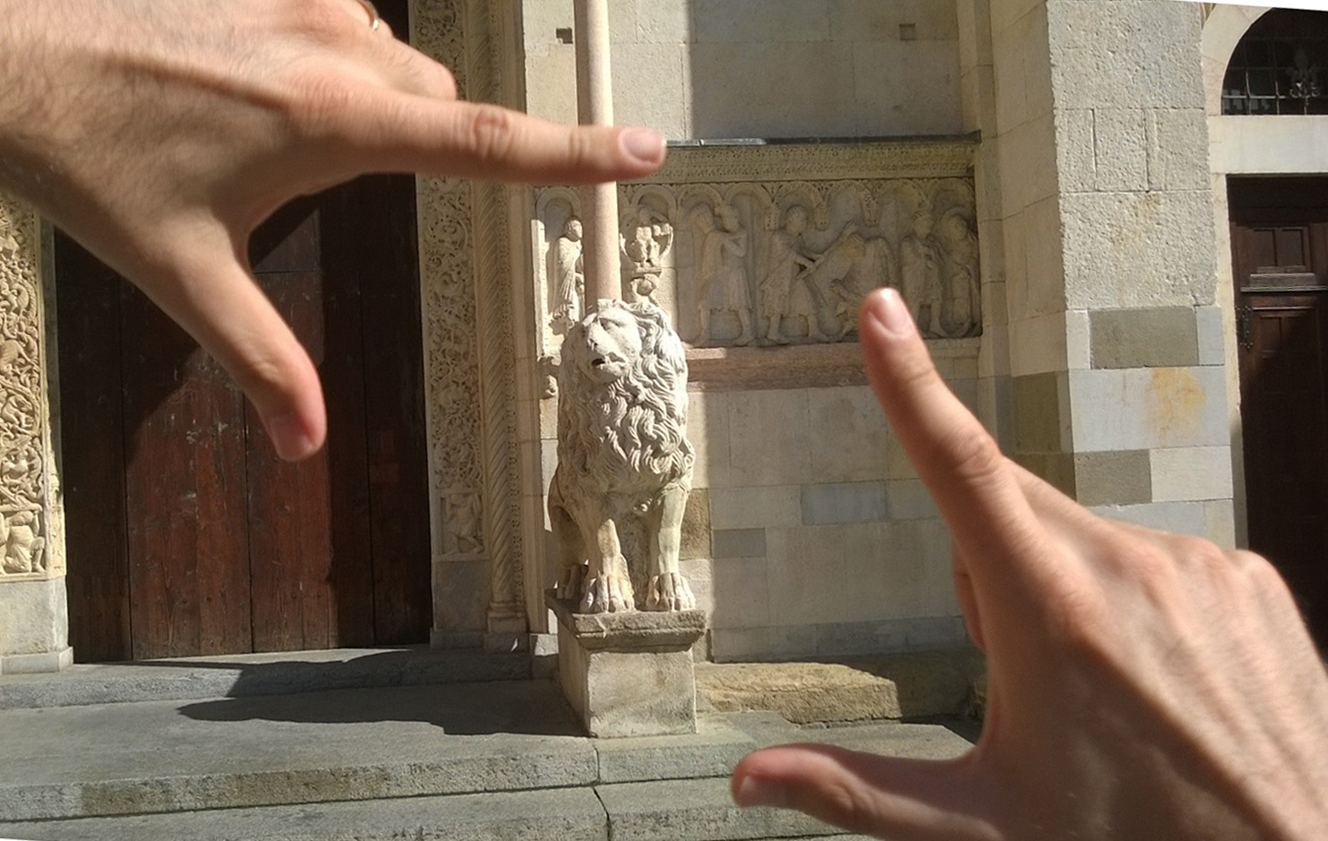
\includegraphics[height=100px]{./Figures/egovision_duomo_modena_1.jpg}}
\caption{One of the goals of this thesis: natural interaction with artworks.}
\label{fig:interaction}
\end{figure*}

Gestures are expressive, meaningful body motions involving physical movements of the fingers, hands, arms, head, face, or
body with the intent of conveying meaningful information or interacting with the environment. They constitute one interesting
small subspace of possible human motion. A gesture may also be perceived by the environment as a compression technique for the information to be transmitted elsewhere and subsequently reconstructed by the receiver. Gesture recognition has wide-ranging applications such as the following:
\begin{itemize}
\item developing aids for the hearing impaired;
\item  enabling very young children to interact with computers;
\item  designing techniques for forensic identification;
\item recognizing sign language;
\item medically monitoring patients’ emotional states or stress
levels;
\item navigating and/or manipulating in virtual environments;
\item communicating in video conferencing;
\item distance learning/tele-teaching assistance;
\item monitoring automobile drivers' alertness/drowsiness
levels, etc.
\end{itemize}

Generally, there exist many-to-one mappings from concepts
to gestures and vice versa. Hence, gestures are ambiguous and
incompletely specified. For example, to indicate the concept
\textit{stop}, one can use gestures such as a raised hand with palm
facing forward, or, an exaggerated waving of both hands over the
head. Similar to speech and handwriting, gestures vary between
individuals, and even for the same individual between different
instances.

Gestures can be static (the user assumes a certain pose or configuration)
or dynamic (with prestroke, stroke, and poststroke
phases). Some gestures also have both static and dynamic elements,
as in sign languages. Again, the automatic recognition
of natural continuous gestures requires their temporal segmentation.
Often one needs to specify the start and end points of a
gesture in terms of the frames of movement, both in time and
in space. Sometimes a gesture is also affected by the context of
preceding as well as following gestures. Moreover, gestures are
often language- and culture-specific.

%----------------------------------------------------------------------------------------

\section{In Closing}
